\documentclass[]{article}
\usepackage{lmodern}
\usepackage{amssymb,amsmath}
\usepackage{ifxetex,ifluatex}
\usepackage{fixltx2e} % provides \textsubscript
\ifnum 0\ifxetex 1\fi\ifluatex 1\fi=0 % if pdftex
  \usepackage[T1]{fontenc}
  \usepackage[utf8]{inputenc}
\else % if luatex or xelatex
  \ifxetex
    \usepackage{mathspec}
  \else
    \usepackage{fontspec}
  \fi
  \defaultfontfeatures{Ligatures=TeX,Scale=MatchLowercase}
\fi
% use upquote if available, for straight quotes in verbatim environments
\IfFileExists{upquote.sty}{\usepackage{upquote}}{}
% use microtype if available
\IfFileExists{microtype.sty}{%
\usepackage{microtype}
\UseMicrotypeSet[protrusion]{basicmath} % disable protrusion for tt fonts
}{}
\usepackage[margin=1in]{geometry}
\usepackage{hyperref}
\hypersetup{unicode=true,
            pdftitle={Predictors of Survival for Titanic Passengers},
            pdfauthor={Alden Chen, Birinder Singh},
            pdfborder={0 0 0},
            breaklinks=true}
\urlstyle{same}  % don't use monospace font for urls
\usepackage{longtable,booktabs}
\usepackage{graphicx,grffile}
\makeatletter
\def\maxwidth{\ifdim\Gin@nat@width>\linewidth\linewidth\else\Gin@nat@width\fi}
\def\maxheight{\ifdim\Gin@nat@height>\textheight\textheight\else\Gin@nat@height\fi}
\makeatother
% Scale images if necessary, so that they will not overflow the page
% margins by default, and it is still possible to overwrite the defaults
% using explicit options in \includegraphics[width, height, ...]{}
\setkeys{Gin}{width=\maxwidth,height=\maxheight,keepaspectratio}
\IfFileExists{parskip.sty}{%
\usepackage{parskip}
}{% else
\setlength{\parindent}{0pt}
\setlength{\parskip}{6pt plus 2pt minus 1pt}
}
\setlength{\emergencystretch}{3em}  % prevent overfull lines
\providecommand{\tightlist}{%
  \setlength{\itemsep}{0pt}\setlength{\parskip}{0pt}}
\setcounter{secnumdepth}{0}
% Redefines (sub)paragraphs to behave more like sections
\ifx\paragraph\undefined\else
\let\oldparagraph\paragraph
\renewcommand{\paragraph}[1]{\oldparagraph{#1}\mbox{}}
\fi
\ifx\subparagraph\undefined\else
\let\oldsubparagraph\subparagraph
\renewcommand{\subparagraph}[1]{\oldsubparagraph{#1}\mbox{}}
\fi

%%% Use protect on footnotes to avoid problems with footnotes in titles
\let\rmarkdownfootnote\footnote%
\def\footnote{\protect\rmarkdownfootnote}

%%% Change title format to be more compact
\usepackage{titling}

% Create subtitle command for use in maketitle
\newcommand{\subtitle}[1]{
  \posttitle{
    \begin{center}\large#1\end{center}
    }
}

\setlength{\droptitle}{-2em}

  \title{Predictors of Survival for Titanic Passengers}
    \pretitle{\vspace{\droptitle}\centering\huge}
  \posttitle{\par}
    \author{Alden Chen, Birinder Singh}
    \preauthor{\centering\large\emph}
  \postauthor{\par}
      \predate{\centering\large\emph}
  \postdate{\par}
    \date{2018-11-17}


\begin{document}
\maketitle

\subsection{Introduction}\label{introduction}

In this analysis, we look at data on passengers from the Titanic. Using
seven features, we fit a decision tree model to find out which two
features are the best predictors of survival for Titanic passengers.

\subsection{Exploratory Data Analysis:}\label{exploratory-data-analysis}

Our target variable is \texttt{Survived}, a dummy variable that takes
the value \texttt{0} is a passenger did not survive and \texttt{1} is he
or she did survive. We have data on 712 passengers for these seven
features

\begin{longtable}[]{@{}ll@{}}
\toprule
Feature & Description\tabularnewline
\midrule
\endhead
Passenger Class & First, Second or Third Class\tabularnewline
Sex & Male or Female\tabularnewline
Age & Age of each passenger years\tabularnewline
Siblings/Spouses & Number of siblings and spouses aboard the
Titanic\tabularnewline
Parents/Children & Number of parents and children aboard the
Titanic\tabularnewline
Fare & The amount each passenger paid for a his or her
ticket\tabularnewline
Port of Embarkation & Cherbourg, Queenstown, or
Southampton\tabularnewline
\bottomrule
\end{longtable}

In this section, we look at some plots of the data and discuss their
implications for prediction.

\emph{Figure 1: Bar Plots, Number of Survivors by Passenger Class, Sex,
and Port of Embarkation}
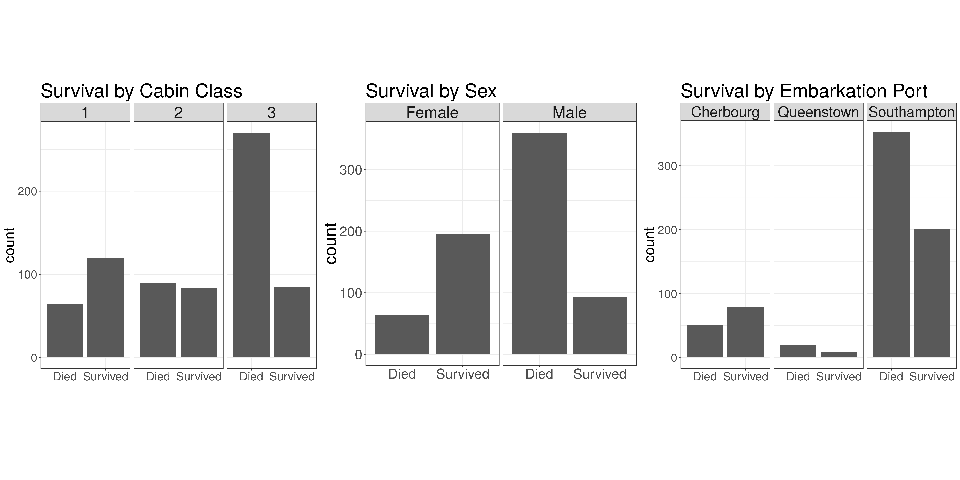
\includegraphics{report_titanic-predictors_files/figure-latex/unnamed-chunk-1-1.pdf}

In the three bar plots above, we compare the number of people who
survived based on passengers' sex, port of embarkation, and cabin class.
We can see that there appears to be a large difference between in the
number of passengers that survived based on sex. For female passengers,
there are more passengers who survived than passengers than died, while
the opposite is true for male passengers. We see a similar trend for
cabin class. Among first class passengers, there are more survivors than
non-survivors, while among third class passengers, there are many more
non-survivors than survivors.This suggests that sex and passenger class
could be important features for predicting survival.

For port of embarkation, the vast majority of passengers boarded at
Southampton, which appears to have similar rates to Queenstown
passengers. Cherbourg passengers seem to have a much higher survival
rate than passengers who boarded at other ports. Given the small number
of Cherbourg passengers, it is unclear if port of embarkation will be a
good predictor of survival.

\emph{Figure 2: Box Plots, Survival vs Age and Survival vs Fare}\\
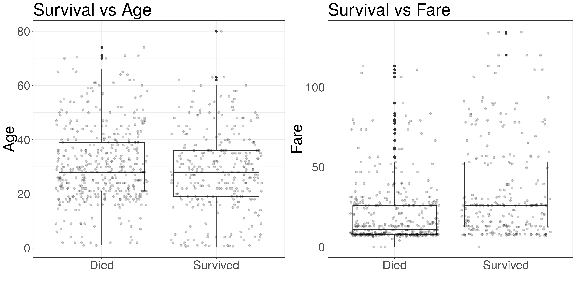
\includegraphics{report_titanic-predictors_files/figure-latex/unnamed-chunk-2-1.pdf}

The box plots above show the distribution of ages and fares of the
passengers based on whether or not they survived. There does not seems
to be only a small difference in the ages of passengers who survived and
those who did not, so age likely would not be a very important feature
for predicting survival.

For fare, it appears that passengers who survived paid higher fares.
This is likely related to the trend that there were more first class
survivors than second or third class survivors. Presumably, first class
passengers paid higher fares, so it is not surprising that survivors on
average paid higher fares.

\subsection{Model Development}\label{model-development}

To decide on the appropriate depth of the tree, we used five-fold cross
validation. Below is a plot of the validation performance for different
depths of trees. We can see a clear spike in the average accuracy at a
depth of 3.

\emph{Figure 3: Validation Performance, 5-Fold Cross Validation}\\
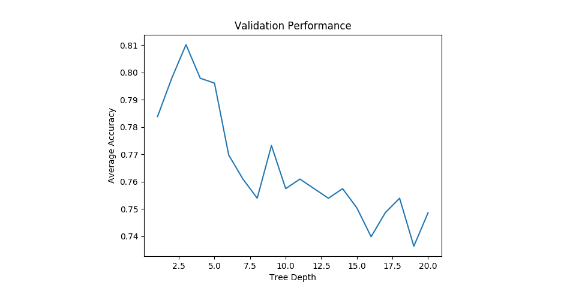
\includegraphics{report_titanic-predictors_files/figure-latex/unnamed-chunk-3-1.pdf}

\subsection{Results}\label{results}

After fitting a model of depth three, we looked at the feature
importances of our model. The plot below summarizes our results. We can
see that the two best predictors of survival for Titanic passengers are
sex and passenger class. This supports our initial observations from the
exploratory plots that we produced.

\emph{Figure 4: Feature Importances}\\
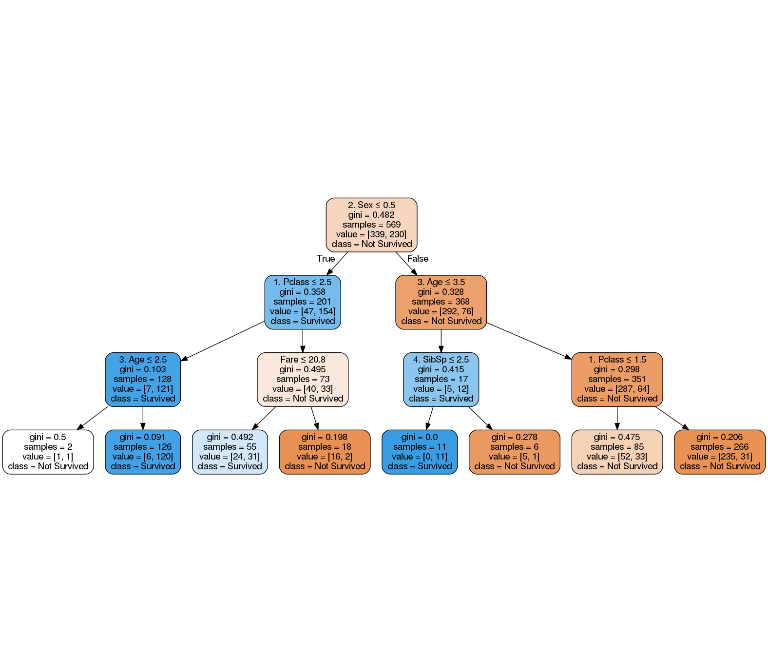
\includegraphics{report_titanic-predictors_files/figure-latex/unnamed-chunk-4-1.pdf}

\subsection{References}\label{references}

Kaggle.(2012). \emph{Titanic: Machine Learning from Disaster} {[}Data
files and description{]}. Retrieved from:
\url{https://www.kaggle.com/c/titanic}

scikit-learn developers. (2018).
\emph{sklearn.tree.DecisionTreeClassifier}. Retrieved from:\\
\url{https://scikit-learn.org/stable/modules/generated/sklearn.tree.DecisionTreeClassifier.html}


\end{document}
